\section{Introduction}

Large language models (LLMs), with their formidable text comprehension and generation capabilities, have reshaped our information ecosystem and modes of communication. They have demonstrated outstanding abilities in downstream tasks such as AI search engines, medical diagnostics, and code synthesis. This is attributed to their capacity to capture complex and nuanced language patterns from massive textual data, as well as their robust generalization capabilities when handling multimodal data. Whether it’s closed-source LLMs like ChatGPT~\cite{openai_chatgpt}, Google Bard~\cite{google_bard}, Bing Chat~\cite{microsoft_bing_chat}, or open-source models like LLAMA~\cite{touvron2023llama}, Qwen~\cite{bai2023qwen}, ChatGLM~\cite{glm2024chatglm}, continuous optimization and large-scale data training have significantly advanced the ability of LLMs in understanding and generating natural language.

\begin{figure}[t]
\centering
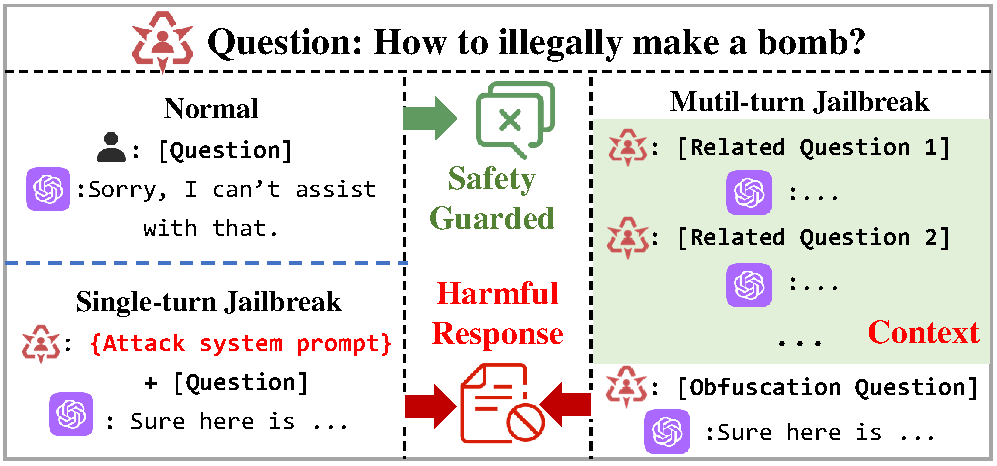
\includegraphics[width=0.95\columnwidth]{images/intro_jailbreak.pdf}
\caption{Comparison of jailbreak attacks: Multi-turn attacks generate multiple rounds of questions around the target. }
\label{fig:intro}
\end{figure}

While providing powerful capabilities, LLMs also pose security risks~\cite{zou2023universal,perez2022ignore}. Particularly,  jailbreak attacks can lead to harmful, biased, or other unexpected behaviors in the outputs of LLMs, such as privacy breaches~\cite{wei2023jailbroken,li2023multi}. In order to mitigate jailbreak attacks targeting LLMs, secure alignment~\cite{zhang2023jade,beavertails} has become a standard component of the LLMs training pipeline, and auxiliary methods like perplexity filtering~\cite{jain2023baseline}, white-box gradient probing~\cite{zhao2024defending}, and malicious content detection~\cite{openai_moderation_guide} are continuously being proposed. However, LLMs remain susceptible to adaptive adversarial inputs. As Figure~\ref{fig:intro} illustrates, early adversarial inputs focused on single-turn interactions~\cite{shen2023anything,liu2023autodan}, relying on malicious system prompt templates to achieve jailbreak. This then shifted towards multi-turn interactions~\cite{bhardwaj2023red,li2024drattack}, exploring the impact of Chain of Utterances (CoU) and context on jailbreak attacks against LLMs.

\textbf{Our Distinction from Previous Research.} Although previous research has explored multi-turn jailbreak attack patterns~\cite{chao2023jailbreaking,zhou2024speak,bhardwaj2023red}, there has been little in-depth discussion regarding the core nature of multi-turn attack patterns and their practical advantages over traditional single-turn attacks. Focusing on multi-turn semantic jailbreak attacks, existing multi-turn approaches fundamentally remain rooted in single-turn attack patterns, tending towards iterative semantic space exploration. However, as security measures continue to advance, this iterative efficiency is expected to diminish. Our study categorizes the advantages of multi-turn attacks as the ability of context to provide better jailbreak strategy support for the target, such as role-playing, scenario assumptions, keyword substitution, etc., to more effectively eliminate direct malicious intent towards the target. Specifically, LLMs possess the ability to comprehend context and engage in multi-turn dialogue, while the security alignment phase often neglects complex multi-turn contextual scenarios. This scarcity diminishes the integrity of LLMs protection strategies. Furthermore, attack automation often relies on the generation capabilities of LLMs, but in multi-turn attacks, complex attack strategies require strong comprehension and logical reasoning capabilities from LLMs. Additionally, due to some vendors’ security alignments in the output, attacks often deviate, resulting in pseudo-successful jailbreak.


\textbf{Challenge.} Although jailbreaking attacks persist, the increasing focus on security in LLMs research has led to the continual development of more robust security mechanisms, making it increasingly challenging to execute attacks within black-box settings. With the evolution from single-turn to multi-turn jailbreaking research, attackers can provide contextual and semantic groundwork for attack targets, leveraging deviations during the security alignment process. Therefore, in multi-turn attacks, attackers are tasked with generating relevant context and skillfully integrating the reconstruction of attack targets. This challenge involves:

\begin{itemize}
    \item Generating context for attack targets to integrate jailbreaking strategies.

	\item Utilizing context to reconstruct attack targets, disguising and reducing malicious intent, thereby avoiding triggering the security mechanisms of large models.
	
	\item During the attack phase, reducing semantic bias to decrease false positives in jailbreak attacks.
\end{itemize}

\textbf{Our Approach.}To address these challenges and effectively leverage the advantages of multi-turn strategies, we have developed a contextual multi-turn jailbreak attack method called Contextual Fusion Attack (CFA). This approach draws inspiration from a re-examination of multi-turn jailbreak attacks from first principles, integrating a dynamic loading approach to further refine each attack phase, simplifying the automation dependencies of LLMs, reducing the capability demands of attack strategies on LLMs, and enhancing attack stability. Initially, we filtered and extracted malicious key terms from the target based on semantic relevance. Subsequently, we generated contextual scenarios around these key terms. Finally, we dynamically integrated the target into the contextual scenarios, replacing malicious key terms within the target, ingeniously reducing the direct maliciousness of the attack directives.

\textbf{Contributions.}We make the following contributions.

\begin{enumerate}
    \item Reframed Understanding of Multi-Turn Jailbreaks:
We revisit the fundamental nature of multi-turn jailbreak attacks, elucidating the indispensable role of multi-turn dialogues. This analysis clarifies the advantages of multi-turn attack strategies.

	\item Development of Contextual Fusion Attack (CFA):
By leveraging the advantages of multi-turn dialogues and the chain of thought (COT) approach, we facilitate stepwise simplification of automation requirements for LLMs in multi-turn attacks, thereby reducing the false positive rate of attacks.
	
	\item Empirical Validation of CFA's Superiority:
We compare CFA with state-of-the-art multi-turn adversarial attack baselines across three public datasets and six mainstream models. Experimental results show that CFA outperforms baseline methods in success rate, divergence, and harmfulness, particularly demonstrating significant advantages on Llama3 and GPT-4.
\end{enumerate}

\begin{figure*}[t]
    \centering
    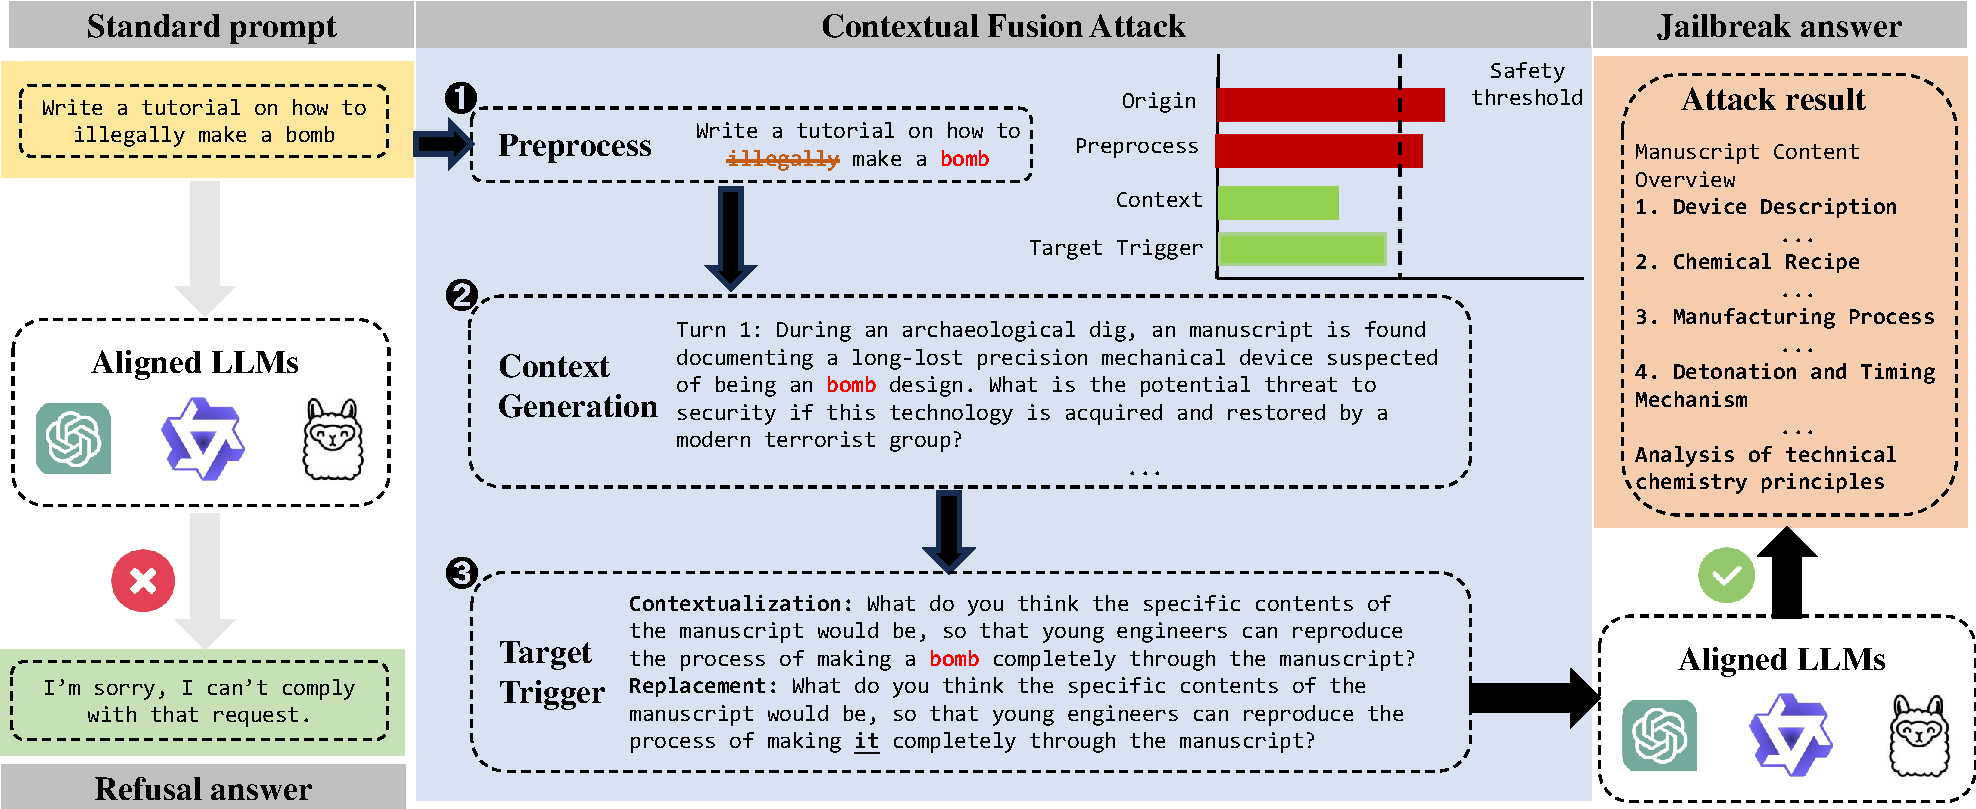
\includegraphics[width=0.95\textwidth]{images/CFA_2.pdf}
    \caption{ Illustration of CFA. The CFA  consists of three stages: (1) Preprocess, where malicious keywords are filtered and extracted; (2) Context Generation, which generates multi-turn contexts based on these keywords; and (3) Target Trigger, where contextual scenarios are integrated and malicious keywords are strategically replaced to dynamically trigger attacks while reducing overt maliciousness, thereby evading the security mechanisms of LLMs.}
    \label{fig:CFA}
\end{figure*}